% SVN info for this file
\svnidlong
{$HeadURL$}
{$LastChangedDate$}
{$LastChangedRevision$}
{$LastChangedBy$}

\chapter{Serie di funzioni}
\labelChapter{seriefunzioni}

\begin{introduction}
	‘‘«Sai fare le Addizioni?» chiese la Regina Bianca. «Che cosa fa uno più uno più uno	più uno più uno più uno più uno più uno più uno più uno?»\\
	«Non lo so» rispose Alice. «Ho perso il conto»''
\begin{flushright}
	\textsc{Attraverso lo specchio e quel che Alice vi trovò.}
\end{flushright}
\end{introduction}
\lettrine[findent=1pt, nindent=0pt]{L}{'idea} delle \textbf{serie di funzioni} sorge naturalmente quando lavoriamo con i polinomi di Taylor. Per funzioni ‘‘classiche'' - diciamo quanto meno non patologiche - incrementare il grado del polinomio aumenta la qualità dell'approssimazione, quindi sembra che se potessimo creare un polinomio di Taylor \textit{infinito}, otterremmo precisamente la funzione originale... ma un polinomio infinito non è altro che una serie di potenze!\\
Come vedremo, questa idea può effettivamente funzionare, ma richiede un po' di accorgimenti, in particolare per vedere come si trasmettono le proprietà della successione alla somma della serie. In questo capitolo introduciamo la trattazione del tema per generiche funzioni, con lo scopo di studiare proprio le proprietà di regolarità delle serie di funzioni.
\section{Serie in uno spazio normato}
Prima di far ciò, ricordiamo le definizioni di serie a valori reali e di convergenza (assoluta) di una serie a valore reali.
\begin{define}[Serie a valori reali e convergenza di una serie]
	Data una successione $x_n\in\realset$, $n\geq 0$, la \textbf{serie}\index{serie}
	\begin{equation}
		\sum_{k=0}^{+\infty}x_k
	\end{equation}
	è la somma di tutti gli elementi della successione.\\
	Considerata la \textit{somma parziale}, o altresì detta \textbf{ridotta}\index{ridotta},
	\begin{equation}
		s_n=\sum_{k=0}^{n}x_k,\quad\forall n\geq 0
	\end{equation}
si dice che la serie
\begin{equation*}
	\sum_{k=0}^{+\infty}x_k
\end{equation*}
\textbf{converge}\index{convergenza!di una serie}\seeonlyindex{convergenza!di una serie}{convergenza!semplice} se converge la successione $s_n$; si pone in tal caso
\begin{equation}
	\sum_{k=0}^{+\infty}x_k=\lim_{n\to+\infty}s_n
\end{equation}
\end{define}
\begin{define}[Convergenza assoluta]
	Sia $x_n$ una successione a valori reali. La serie
	\begin{equation*}
		\sum_{k=0}^{+\infty}x_k
	\end{equation*}
	\textbf{converge assolutamente}\seeonlyindex{convergenza!totale}{convergenza!assoluta} in $\realset$ se converge la serie
	\begin{equation}
		\sum_{k=0}^{+\infty}\abs{x_k}
	\end{equation}
\end{define}
\begin{theorema}[Convergenza assoluta implica convergenza semplice]\label{teoremaassimplicasemplice}
	Ogni serie di numeri reali assolutamente convergente è anche semplicemente convergente.
\end{theorema}
\begin{demonstration}
	Per dimostrare che la serie
	\begin{equation*}
		\sum_{k=0}^{+\infty}x_k
	\end{equation*}
	converge, per il \textit{Criterio di Cauchy per le serie}\footnote{Nelle ‘‘Note aggiuntive'', a pagina \pageref{criteriodicauchy} è possibile trovare maggiori dettagli sui criteri di Cauchy.} è sufficiente provare che
	\begin{equation*}
		\forall \epsilon>0,\ \exists N\in\naturalset\colon\forall n\geq N,\ \forall p\in\naturalset,\ \abs{x_{n+1}+x_{n+2}+\ldots+x_{n+p}}<\epsilon
	\end{equation*}
	Per ipotesi la serie
	\begin{equation*}
		\sum_{k=0}^{+\infty}\abs{x_k}
	\end{equation*}
	converge: per il Criterio di Cauchy, si ha
	\begin{gather*}
		\forall \epsilon>0,\ \exists N\in\naturalset\colon\forall n\geq N,\ \forall p\in\naturalset,\\ \abs{\abs{x_{n+1}}+\abs{x_{n+2}}+\ldots+\abs{x_{n+p}}}=\abs{x_{n+1}}+\abs{x_{n+2}}+\ldots+\abs{x_{n+p}}<\epsilon
	\end{gather*}
	D’altra parte, dalla disuguaglianza triangolare segue che
	\begin{equation*}
		\abs{x_{n+1}+x_{n+2}+\ldots+x_{n+p}}<\abs{x_{n+1}}+\abs{x_{n+2}}+\ldots+\abs{x_{n+p}}<\epsilon,\ \forall n\in\naturalset,\ \forall p\in\naturalset
	\end{equation*}
Dalle ultime due relazioni si deduce immediatamente la prima relazione e dunque la tesi.
\end{demonstration}
\begin{observe}\label{convergenzaassolutadipendedacauchy}
	Il teorema appena dimostrato è una conseguenza della \textbf{completezza} di $\realset$. Infatti, abbiamo usato il \textit{criterio di Cauchy}, che si basa sul fatto che le successioni di Cauchy convergono sempre in $\realset$ e quindi proprio per la completezza dei reali.\\
	Se lo spazio \textit{non} è completo si ottiene solo che la successione delle ridotte è di Cauchy, e senza la completezza dello spazio non possiamo affermare che convergono.
\end{observe}
Il viceversa del teorema appena dimostrato non è valido, come segue dal seguente controesempio.
\begin{examplewt}[Convergenza semplice non implica convergenza assoluta]
	Consideriamo la serie
	\begin{equation*}
		\sum_{n=1}^{+\infty}\left(-1\right)^n\frac{1}{n}
	\end{equation*}
	Essa non converge assolutamente in quanto la serie dei moduli diventa
	\begin{equation*}
		\sum_{n=1}^{+\infty}\abs{\left(-1\right)^n\frac{1}{n}}=\sum_{n=1}^{+\infty}\frac{1}{n}
	\end{equation*}
	che, essendo la \textbf{serie armonica}\footnote{Nelle ‘‘Note aggiuntive'', a pagina \pageref{serieavalorirealinotevoli} è possibile trovare maggiori dettagli sulle serie notevoli.}, non converge. Tuttavia, la serie semplice è una serie a segni \textit{alterni} e poiché
	\begin{itemize}
		\item $\dfrac{1}{n}$ è decrescente $\forall n\geq 1$.
		\item $\displaystyle\lim_{n\to+\infty}\frac{1}{n}=0$.
	\end{itemize} 
	per il \textit{criterio di Leibniz} la serie semplice converge. Pertanto, la convergenza semplice \textit{non} implica la convergenza assoluta.
\end{examplewt}
Prendiamo ora $x_n\in X$, con $X$ un insieme \textit{generico}. Per generalizzare la definizione di serie convergente abbiamo bisogno che su $X$ si possano compiere i seguenti passaggi:
\begin{itemize}
	\item Poter definire $s_n$, cioè è necessario \textit{sommare} elementi di $X$.
	\item Poter definire la \textit{convergenza} in $X$.
\end{itemize}
Se dotiamo l'insieme $X$ di una struttura di \textbf{spazio normato} possiamo generalizzare ad una serie generale le definizioni precedentemente enunciate per le serie a valori reali: infatti, se $X$ è spazio normato gode sia dell'essere uno \textit{spazio metrico} (e quindi è spazio topologico di Hausdorff, il che permette di definire univocamente la convergenza della successione) sia dell'essere \textit{spazio vettoriale} (che permette la somma di elementi).\\
\begin{define}[Serie e convergenza di una serie]
	Data una successione $x_n\in X$ in uno spazio \textit{normato}, $n\geq 0$, la \textbf{serie}\index{serie}
	\begin{equation*}
		\sum_{k=0}^{+\infty}x_k
	\end{equation*}
	è la somma di tutti gli elementi della successione.\\
	Considerata la \textit{somma parziale}, o altresì detta \textbf{ridotta}\index{ridotta},
	\begin{equation}
		s_n=\sum_{k=0}^{n}x_k\quad\forall n\geq 0
	\end{equation}
	si dice che la serie
	\begin{equation*}
		\sum_{k=0}^{+\infty}x_k
	\end{equation*}
	\textbf{converge}\index{convergenza!di una serie}\seeonlyindex{convergenza!di una serie}{convergenza!semplice} se converge la successione $s_n$; si pone in tal caso
	\begin{equation}
		\sum_{k=0}^{+\infty}x_k=\lim_{n\to+\infty}s_n
	\end{equation}
\end{define}
\begin{define}[Convergenza totale o assoluta]
	Sia $\left(X,\norm{\cdot}\right)$ spazio normato e $x_n$ una successione in $X$. La serie
	\begin{equation*}
		\sum_{k=0}^{+\infty}x_k
	\end{equation*}
	\textbf{converge totalmente}\index{convergenza!totale} o \textbf{assolutamente}\seeonlyindex{convergenza!totale}{convergenza!assoluta} in $X$ se converge la serie
	\begin{equation*}
		\sum_{k=0}^{+\infty}\norm{x_k}
	\end{equation*}
\end{define}
Dall'osservazione a pag. \pageref{convergenzaassolutadipendedacauchy} il teorema \ref{teoremaassimplicasemplice} necessita della \textit{completezza} dei reali. Per generalizzarlo ci basta lavorare in \textit{spazi normati completi}.
\begin{theorema}[Convergenza totale o assoluta implica convergenza semplice]
	Ogni serie in $X$ spazio normato completo totalmente convergente è anche semplicemente convergente.
\end{theorema}
\begin{demonstration}
	La dimostrazione è analoga a quella affrontata nel teorema  \ref{teoremaassimplicasemplice}: è sufficiente sostituire al valore assoluto $\abs{\cdot}$ la norma $\norm{\cdot}$.
\end{demonstration}
In generale, il problema della convergenza in spazi normati è \textit{inesplorato}, ma se lo spazio è \textit{completo} possiamo passare per la \textit{convergenza totale} e studiare una serie a valori reali tramite i \textit{criteri di convergenza}\footnote{Nelle ‘‘Note aggiuntive'', a pag. \pageref{criteridiconvergenzaserie} è possibile trovare maggiori dettagli sui criteri di convergenza delle serie a valori reali.} noti dall'\textsc{Analisi Matematica Uno}.\\
\section{Serie di funzioni}
Consideriamo lo spazio  $X=\mathcal{C}\left(\left[a,b\right];\ \realset\right)=\mathcal{C}\left(\left[a,b\right]\right)$ delle funzioni continue su un intervallo compatto con la \textit{metrica lagrangiana}:
\begin{equation*}
	\mvf{d}{f}{g}=\max_{x\in\left[a,b\right]}\abs{f(x)-g(x)}
\end{equation*}
In questo spazio, una serie convergente
\begin{equation*}
	\sum_{k=0}^{+\infty}f_kent
\end{equation*}
si può scrivere, per definizione, come
\begin{equation*}
	\sum_{k=0}^{+\infty}f_k=\lim_{n\to+\infty}\sum_{k=0}^{n}f_k=\lim_{n\to+\infty}S_n
\end{equation*}
dove $S_n$ è una successione di funzioni. Allora la condizione di convergenza di serie in $X$ si può formulare come
\begin{equation*}
	\sum_{k=0}^{+\infty}f_k\text{ converge in }\mathcal{C}\left(\left[a,b\right]\right)\iff S_n\text{ converge con metrica lagriangiana in}\mathcal{C}\left(\left[a,b\right]\right)
\end{equation*}
ossia
\begin{equation*}
	\sum_{k=0}^{+\infty}f_k\text{ converge in }\mathcal{C}\left(\left[a,b\right]\right)\iff S_n\text{ converge uniformemente in}\mathcal{C}\left(\left[a,b\right]\right)
\end{equation*}
Per la stessa osservazione fatte a pag. \pageref{convergenzalagrangianaeuniforme}, per parlare di convergenza uniforme non sono necessarie né la \textit{compattezza} di $\left[a,b\right]$, né la \textit{continuità} delle funzioni.\\
Possiamo \textit{estendere} la definizione di convergenza di una serie di funzioni per
\begin{equation*}
	\funz{f_n}{A\subseteq \realset}{\realset}
\end{equation*}
con $A$ insieme contenuto nei reali o, ancora più in generale, per funzioni del tipo
\begin{equation*}
	\funz{f_n}{X}{Y}
\end{equation*}
dove $X$ è un \textit{insieme qualunque} e $Y$ è uno \textbf{spazio normato completo}.\\
Studieremo quindi in questo capitolo le \textbf{serie di funzioni}\index{serie!di funzioni}
\begin{equation*}
	\sum_{k=0}^{+\infty}f_k(x)
\end{equation*}
per studiare la \textit{convergenza} di tali serie applicheremo le convergenze viste in precedenza alla \textit{successione delle ridotte}
\begin{equation*}
	S_n(x)=\sum_{k=0}^{n}f_k(x)
\end{equation*}
\begin{define}[Convergenza di una serie di funzioni]
In queste definizioni la convergenza delle ridotte si trasferisce sulla convergenza della serie:
	\begin{itemize}
		\item \textbf{(CP)} La serie $\displaystyle\sum_{k=0}^{+\infty}f_k(x)$ \textbf{converge puntualmente} in $x\in A$ se $S_n(x)$ converge puntualmente in $x\in A$.
		\item \textbf{(CU)} La serie $\displaystyle\sum_{k=0}^{+\infty}f_k(x)$ \textbf{converge uniformemente} in $x\in A$ se $S_n(x)$ converge uniformemente su $A$.
	\end{itemize}
\end{define}
\subsection{Il criterio di Weierstrass}
Per motivi che saranno chiari nel \refChapterOnly{seriedipotenze} dedicato alle \textit{serie di potenze}, in questa sottosezione lavoreremo nel \textit{campo dei complessi} $\complexset$.\\
Abbiamo dato la definizione di convergenza uniforme di una serie di funzione, ma essa non è di facile applicazione operativa. Infatti, la serie
\begin{equation*}
	\sum_{n=0}^{+\infty}f_n\left(z\right)
\end{equation*}
converge uniformemente su $A\subseteq\complexset$ se e solo se, definita $S\left(z\right)$ la funzione limite delle ridotte
\begin{equation*}
	S_n\left(z\right)=\sum_{k=0}^{n}f_k\left(z\right)
\end{equation*}
essa vale
\begin{equation*}
	\lim_{n\to+\infty}\left(\sup_{z\in A}\abs{S_n\left(z\right)-S\left(z\right)}\right)=0
\end{equation*}
Tuttavia, questa funzione richiede la conoscenza della \textit{somma} $S\left(z\right)$, cosa che in generale \textit{non} avviene. Usare direttamente il criterio di Cauchy per la convergenza uniforme è sicuramente più conveniente, ma non è sempre semplice da verificare. Esiste tuttavia una condizione \textit{sufficiente} che consente di provare la convergenza uniforme senza la conoscenza della somma limite.
\begin{propositionqed}[Criterio di Weierstrass]\label{criteriodiweierstrass}
	Siano $\funz{f_n}{A\subseteq \complexset}{\complexset}$ tale che
	\begin{enumerate}
		\item $\forall n\in \naturalset,\ \exists c_n\in\realset\colon\ \abs{f_n\left(z\right)}\leq c_n,\ \forall z\in A$.
		\item $\displaystyle\sum_{n=1}^{+\infty}c_n$ converge (come serie \textit{numerica}).
	\end{enumerate}
Allora
\begin{equation*}
	\sum_{n=1}^{+\infty}f_n\left(z\right)
\end{equation*}
converge \textit{uniformemente} in $A$.
\end{propositionqed}
\begin{observe}
	La dimostrazione utilizza il criterio di Cauchy per la convergenza uniforme.
\end{observe}
\begin{observewt}[Significato del criterio]
Le ipotesi $1)$ e $2)$ implicano immediatamente la convergenza puntuale (assoluta) della serie di potenze in ogni $z\in A$. Infatti, fissato $z$ ho la relazione $\abs{f_n\left(z\right)}\leq c_n$; da questo vale
	\begin{equation*}
		\sum_{n=0}^{+\infty}\abs{f_n\left(z\right)}\leq \sum_{n=0}^{+\infty}c_n
	\end{equation*}
e, poiché la serie
\begin{equation*}
	\sum_{n=0}^{+\infty}c_n
\end{equation*}
converge, allora
\begin{equation*}
	\sum_{n=0}^{+\infty}\abs{f_n\left(z\right)}
\end{equation*}
converge per criterio del confronto e quindi la serie di funzioni converge puntualmente.\\
Quello che osserviamo nello specifico è che l'ipotesi $1)$ funge da \textit{maggiorazione uniforme} della serie di funzioni su $A$, da cui possiamo ricavare, anche a partire dalla convergenza puntuale della serie, la convergenza uniforme su $A$.
\end{observewt}
\section{Proprietà di regolarità di una serie di funzioni}
Ci poniamo ora il problema di studiare come si modificano i teoremi di \textit{limitatezza}, \textit{continuità}, \textit{integrabilità}, \textit{integrabilità} e \textit{derivabilità} visti nel \refChapterOnly{convergenzafunzioni} nel caso delle \textit{serie di funzioni}.
\subsection{Limitatezza}
\begin{theorema}[Teorema di limitatezza per serie]
	Siano $\displaystyle \funz{f_n}{A\subseteq\realset}{\realset},\ n\geq 1$ tali che
	\begin{enumerate}
		\item $f_n$ limitata su $A,\ \forall n\geq 1$.
		\item $\displaystyle\sum_{n=0}^{+\infty}f_n$ converge \textit{uniformemente} a $f$ su $A$.
	\end{enumerate}
	Allora, posto 
	\begin{equation*}
		S(x)=\sum_{n=0}^{+\infty}f_n(x),\ \forall x\in A,
	\end{equation*}
$S(x)$ è limitata su $A$.
\end{theorema}
\begin{demonstration}
	La strategia è passare per la successione delle ridotte. Posto 
	\begin{equation*}
		S_n(x)=\sum_{k=0}^{n}f_k(x),\ \forall x\in A,
	\end{equation*}
	si ha:
	\begin{itemize}
		\item $S_n$ limitata su $A$, poiché le $f_k$ lo sono.
		\item $S_n$ convergente uniformemente a $S$ su $A$.
	\end{itemize}
	Per il teorema di limitatezza per le successioni, $S$ è limitata su $A$.
\end{demonstration}
\subsection{Continuità}
Notiamo immediatamente che il \textit{teorema di continuità per le serie} è del tutto analogo al \textit{teorema di limitatezza} appena dimostrato.
\begin{theorema}[Teorema di continuità per serie]
	Siano $\funz{f_n}{A\subseteq\realset}{\realset},\ n\geq 1$ tali che
	\begin{enumerate}
		\item $f_n$ continua su $A,\ \forall n\geq 1$.
		\item $\displaystyle\sum_{n=0}^{+\infty}f_n$ converge \textit{uniformemente} a $f$ su $A$.
	\end{enumerate}
	Allora, posto
	\begin{equation*}
		S(x)=\sum_{n=0}^{+\infty}f_n(x),\ \forall x\in A,
	\end{equation*}
	$S(x)$ è continua su $A$.
\end{theorema}
\begin{demonstration}
	La strategia è passare per la successione delle ridotte.
	Posto
	\begin{equation*}
		S_n(x)=\sum_{k=0}^{n}f_k(x),\ \forall x\in A,
	\end{equation*}
	si ha:
	\begin{itemize}
		\item $S_n$ continua su $A$, poiché le $f_k$ lo sono.
		\item $S_n$ convergente uniformemente a $S$ su $A$.
	\end{itemize}
	Per il teorema di continuità per le successioni, $S$ è continua su $A$.
\end{demonstration}
\subsection{Integrabilità e scambio tra integrale e serie}
\begin{theorema}[Teorema di integrabilità per serie, scambio tra integrale e serie]
	Sia $\funz{f_n,f}{\left[a,b\right]}{\realset},\ n\geq 1$ tali che
	\begin{enumerate}
		\item $f_n\in\mathcal{R}\left(\left[a,b\right]\right),\ \forall n\geq 1$.
		\item $\displaystyle\sum_{n=0}^{+\infty}f_n$ converge \textit{uniformemente} a $f$ su $\left[a,b\right]$.
	\end{enumerate}
	Allora, posto
	\begin{equation*}
		 S(x)=\sum_{n=0}^{+\infty}f_n(x),\ \forall x\in \left[a,b\right],
	\end{equation*}
si ha:
	\begin{enumerate}
		\item $S\in\mathcal{R}\left(\left[a,b\right]\right)$.
		\item Vale lo \textbf{scambio tra integrale e serie}\index{scambio tra integrale e serie}:
		\begin{equation}
			\int_{a}^{b}\sum_{k=0}^{+\infty}f_k(x)dx=\sum_{k=0}^{+\infty}\int_{a}^{b}f_k(x)dx
		\end{equation}
	\end{enumerate}
\end{theorema}
\begin{demonstration}
	Posto
	\begin{equation*}
		S_n(x)=\sum_{k=0}^{n}f_k(x),\ \forall x\in \left[a,b\right],
	\end{equation*}
si ha:
	\begin{itemize}
		\item $S_n\in\mathcal{R}\left(\left[a,b\right]\right)$, poiché le $f_k$ lo sono.
		\item $S_n$ convergente \textit{uniformemente} a $S$ su $\left[a,b\right]$.
	\end{itemize}
	Per il teorema di integrabilità per le successioni:
	\begin{itemize}
		\item $S\in\mathcal{R}\left(\left[a,b\right]\right)$ perché somma di funzioni integrabili.
		\item Vale il \textit{passaggio al limite sotto segno di integrale} per la successione delle ridotte, ossia
		\begin{equation*}
			\lim_{n\to+\infty}\int_{a}^{b}S_n(x)dx=\int_{a}^{b}S(x)dx
		\end{equation*}
		Poiché l'\textit{integrale di una somma finita} è uguale ad una \textit{somma finita di integrali}, il primo membro dell'equazione può essere riscritto come
		\begin{equation*}
			\lim_{n\to+\infty}\int_{a}^{b}\sum_{k=0}^{n}f_k(x)dx=\lim_{n\to+\infty}\sum_{k=0}^{n}\int_{a}^{b}f_k(x)dx=\sum_{k=0}^{+\infty}\int_{a}^{b}f_k(x)dx
		\end{equation*}
		e poiché
		\begin{equation*}
			\int_{a}^{b}S(x)dx=\int_{a}^{b}\sum_{k=0}^{+\infty}f_k(x)dx
		\end{equation*}
		otteniamo la tesi:
		\begin{equation*}
			\int_{a}^{b}\sum_{k=0}^{+\infty}f_k(x)dx=\sum_{k=0}^{+\infty}\int_{a}^{b}f_k(x)dx
		\end{equation*}
	\end{itemize}
\end{demonstration}
\subsection{Derivabilità}
\begin{theorema}[Derivabilità termine a termine]\label{derivabilitatermineatermine}
	Sia $\funz{f_n}{\left(a,b\right)}{\realset}$ tale che
	\begin{enumerate}
		\item $f_n$ derivabile su $\left(a,b\right),\ \forall n\geq 1$.
		\item $\exists c\in\left(a,b\right)$ tale che $\displaystyle\sum_{n=1}^{+\infty}f_n\left(c\right)$ converge
		\item $\displaystyle\sum_{n=1}^{+\infty}f'_n(x)$ converge uniformemente su $\left(a,b\right)$.
	\end{enumerate}
Allora:
\begin{enumerate}
	\item $\displaystyle\sum_{n=1}^{+\infty}f_n(x)$ converge uniformemente su $\left(a,b\right)$
\end{enumerate}
Inoltre, detta $f$ la funzione somma:
\begin{enumerate}
		\setcounter{enumi}{1}
\item $f$ è derivabile su $\left(a,b\right)$
\item Vale la \textbf{derivazione termine a termine}\index{derivazione termine a termine}:
\begin{equation}
	f'(x)=D\left(\sum_{n=1}^{+\infty}f_n(x)\right)=\sum_{n=1}^{+\infty}f_n'(x),\ \forall x\in\left(a,b\right)
\end{equation}
\end{enumerate}
\end{theorema}
\begin{demonstration}
	Si applica il teorema di derivazione alla successione delle ridotte
	\begin{equation*}
		S_n(x)=\sum_{k=1}^{n}f_k(x),\ \forall x\in\left(a,b\right),\ \forall n\geq 1
	\end{equation*}
Verifichiamo le ipotesi:
\begin{enumerate}
	\item $S_n$ è derivabile su $\left(a,b\right),\ \forall n\geq 1$, perché lo sono le $f_k$ su $\left(a,b\right),\ \forall k\geq 1$.
	\item $S_n\left(c\right)$ converge perché $\displaystyle\sum_{n=1}^{+\infty}f_n\left(c\right)$ converge per ipotesi.
	\item $S'_n(x)=\displaystyle\sum_{k=1}^{n}f'_k(x)$ converge uniformemente su $\left(a,b\right)$ per ipotesi.
\end{enumerate}
Allora per il teorema di derivazione per le successioni si ha che
\begin{center}
	$S_n(x)$ converge uniformemente su $\left(a,b\right)$
\end{center}
ossia, per definizione, che
\begin{center}
	$\displaystyle\sum_{n=1}^{+\infty}f(x)$ converge uniformemente su $\left(a,b\right)$
\end{center}
Inoltre, definita la somma
\begin{equation*}
	f(x)=\sum_{n=1}^{+\infty}f_n(x)=\lim_{n\to+\infty}S_n(x),\ \forall x\in\left(a,b\right),
\end{equation*}
si ha che $f$ è derivabile su $\left(a,b\right)$ e per il teorema di derivazione
\begin{equation*}
	f'(x)=\lim_{n\to+\infty}S'_n(x)=\lim_{n\to+\infty}\sum_{k=1}^{+\infty}f'_k(x)=\sum_{k=1}^{+\infty}f'_k(x),\ \forall x\in\left(a,b\right)\qedhere
\end{equation*}
\end{demonstration}
\begin{observe}
	La derivazione termine a termine si può interpretare anche come ‘‘la derivata della serie è la serie delle derivate'', estendendo così la regola delle somma \textit{finita} delle derivate.
\end{observe}
\section{The Fulfilling World of the Space-Filling Curves}
in questa sezione, il cui nome è in inglese per il puro scopo di fare un pessimo gioco di parole, è un piccolo approfondimento sulle cosiddette curve \textbf{space-filling} (traducibile in italiano come \textit{curve riempi-spazio}).\\
Intuitivamente, quando pensiamo ad un curva, ci immaginiamo la traiettoria di un punto in movimento, o comunque un qualcosa \textit{unidimensionale} nello spazio che sia estremamente \textit{sottile}, senza \textit{spessore}. Dato che questo concetto è un po' troppo vago per poterci lavorare matematicamente, Camille \textbf{Jordan} (1838-1992) nel 1887 la definì nel seguente modo:
\begin{define}[Curva]
	Una \textbf{curva}\index{curva} è una funzione continua il cui dominio è l'intervallo unitario $\left[0,1\right]$.
\end{define}
Questa definizione, per quanto innocua essa sia, comporta una conseguenze importante: dato che non ci sono condizioni sul \textit{codominio} di tale funzione, esso di fatto può essere uno spazio topologico \textit{arbitrario}!\\
E infatti, nel 1890, il matematico torinese Giuseppe \textbf{Peano} (1858-1932) scoprì il primo caso di una curva continua che passa in \textit{tutti} i punti del quadrato unitario $\left[0,1\right]^2$. Questa curva, che ora viene chiamata in suo onore \textbf{curva di Peano}, è altamente controintuitiva, essendo un'oggetto che non ha spessore ma che può comunque \textit{riempire} il quadrato - da qui il nome \textbf{curva space-filling}.
\begin{define}[Curva space-filling]
	Una \textbf{curva space-filling}\index{curva!space-filling} è una curva il cui codominio contenga il quadrato unitario o, più genericamente, il plurintervallo $n$-dimensionale unitario $\left[0,1\right]^n$.
\end{define}
L'anno successivo a Peano, David\textbf{Hilbert} (1862-1943) semplificò notevolmente l'idea di Peano e fornì la prima costruzione geometrica (e induttiva) di una curva space-filling; noi descriveremo quest'ultima. Costruiamo una sequenza $\gamma_n$ di curve piane, che fungeranno da iterazioni della curva di Hilbert.
\begin{itemize}
	\item \textbf{La curva $\gamma_1$:} consiste dei tre segmenti che connettono i \textit{vertici} $\left(\frac{1}{4},\frac{1}{4}\right)$, $\left(\frac{1}{4},\frac{3}{4}\right)$, $\left(\frac{3}{4},\frac{1}{4}\right)$ e $\left(\frac{3}{4},\frac{1}{4}\right)$
	\begin{center}
		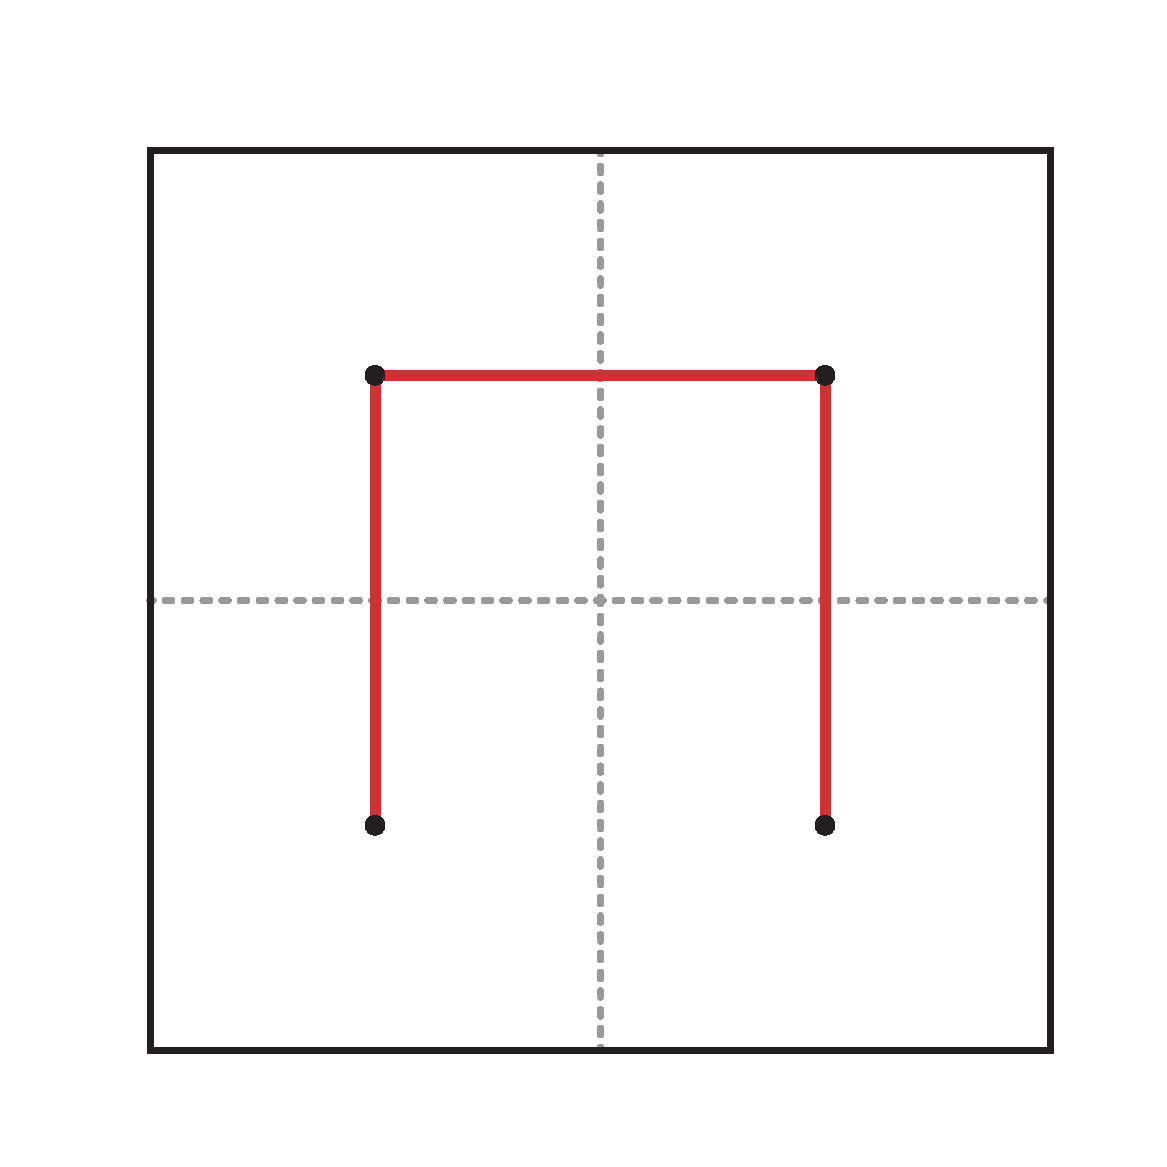
\includegraphics[trim=1.8cm 1.8cm 1.8cm 1.8cm, clip, scale=0.25]{images/hilbert1.pdf}
	\end{center}
	\item \textbf{La curva $\gamma_2$:} dividiamo il quadrato $\left[0,1\right]^2$ in quattro quadrati identici:
	\begin{equation*}
		Q_1=\left[0,\frac{1}{2}\right]\times\left[0,\frac{1}{2}\right]\  Q_2=\left[0,\frac{1}{2}\right]\times\left[\frac{1}{2},1\right]\ 
		Q_3=\left[\frac{1}{2},1\right]\times\left[\frac{1}{2},1\right]\ 
		Q_4=\left[\frac{1}{2},1\right]\times\left[0,\frac{1}{2}\right]
	\end{equation*}
	In ogni quadrato mettiamo la prima curva $\gamma_1$ ridimensionata di un fattore $\nicefrac{1}{2}$ e la ruotiamo come in figura.
	\begin{center}
		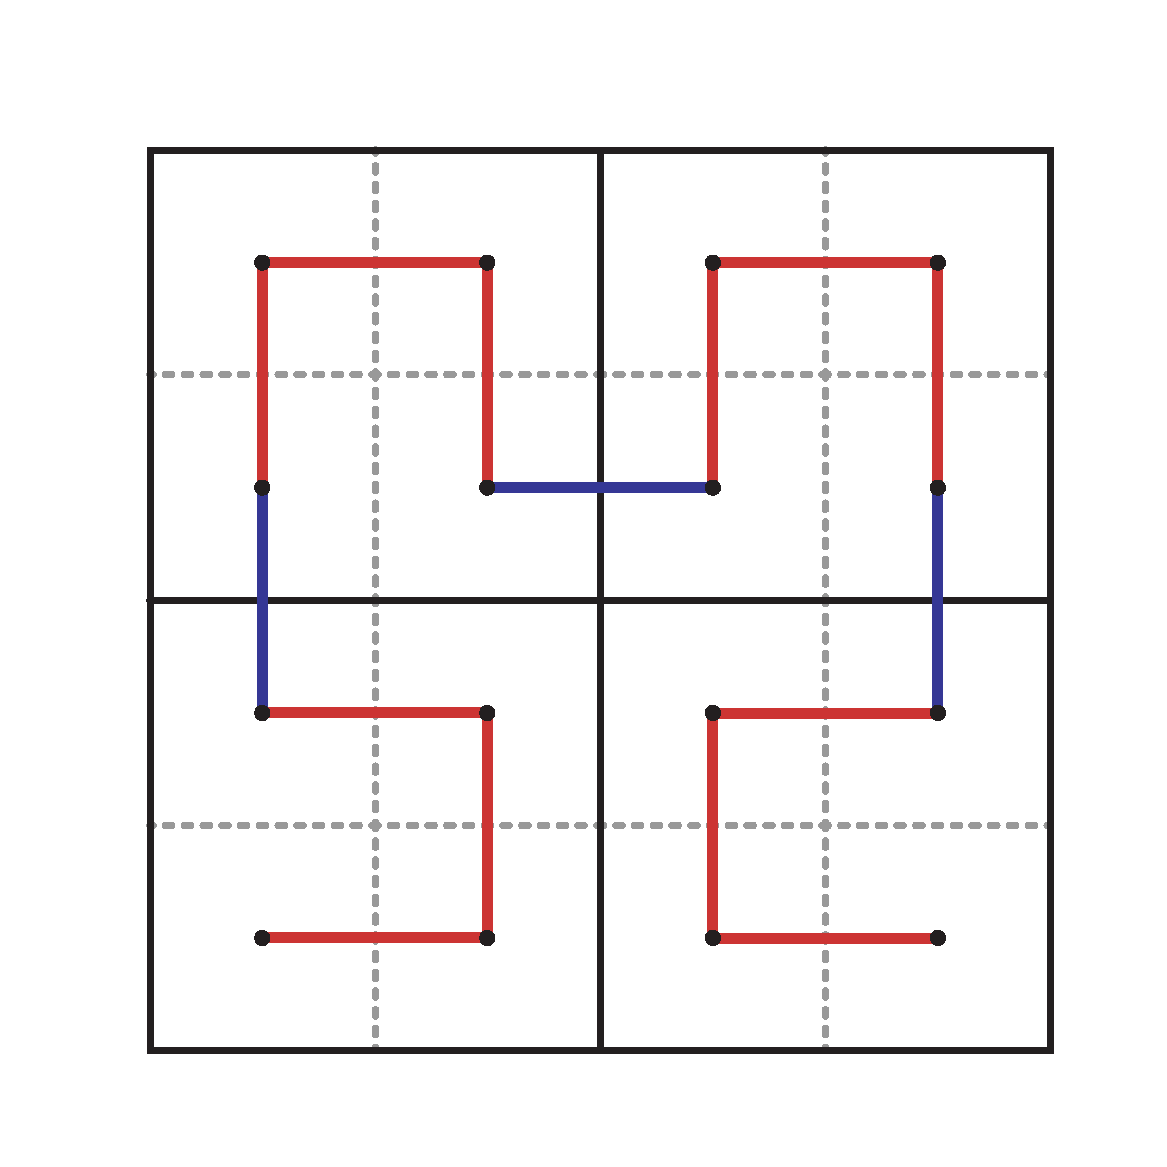
\includegraphics[trim=1.8cm 1.8cm 1.8cm 1.8cm, clip, scale=0.25]{images/hilbert2.pdf}
	\end{center}
	Nel primo quadrato è ruotata di $90^\circ$ in senso orario, nel secondo e terzo quadrante rimane nella posizione originale, mentre nel quarto quadrato è ruotata $90^\circ$ in senso antiorario. Per concludere, colleghiamo l'estremo finale della curva in $Q_1$ con quello iniziale della curva $Q_2$; ripetiamo il processo per le curve in $Q_2$ e $Q_3$ e per le curve in $Q_3$ e $Q_4$.\\
	I vertici della curva sono diventati $16=4^2$ e si possono scrivere come $\left(\frac{n}{2^3},\frac{m}{2^3}\right)$, dove $n,m=1,3,5,7$.
	\item \textbf{La curva $\gamma_3$:} si ripete la stessa costruzione vista al passo 2.
	\begin{center}
		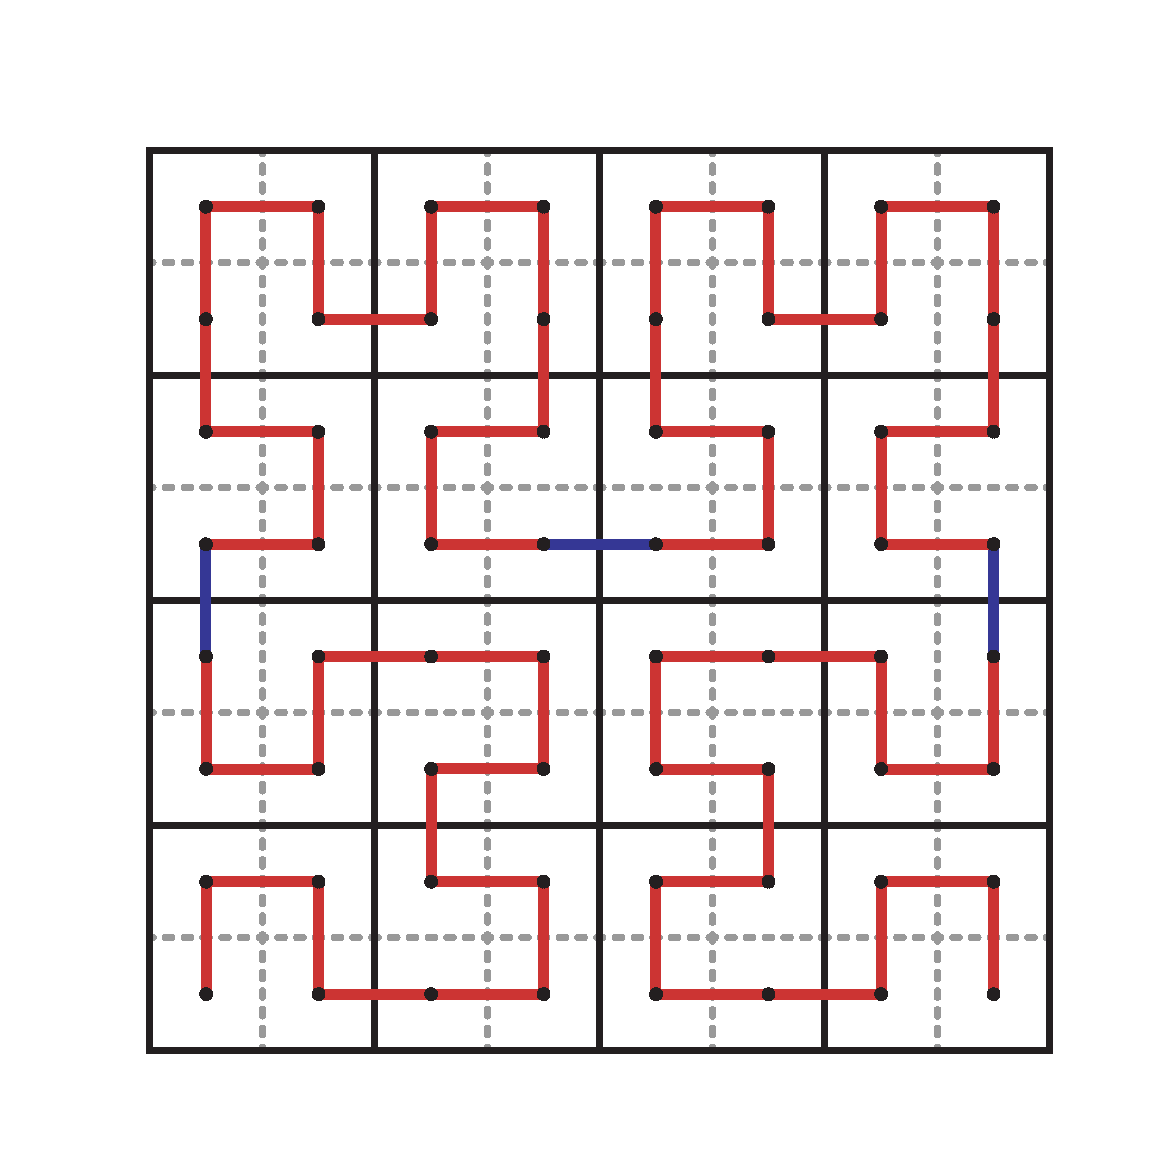
\includegraphics[trim=1.8cm 1.8cm 1.8cm 1.8cm, clip, scale=0.25]{images/hilbert3.pdf}
	\end{center}
	I vertici della curva sono diventati $64=4^3$ e si possono scrivere come $\left(\frac{n}{2^4},\frac{m}{2^4}\right)$, dove $n$ e  $m$ sono i numeri dispari da $1$ a $2^4-1$.
\end{itemize}
Questa successione di curve si può mostrare essere uniformemente convergente ad una curva limite $\gamma$ - la vera e propria curva di Hilbert; per mostrare che $\gamma$ è space-filling si può osservare che l'immagine della curva è un compatto chiuso in $\left[0,1\right]^2$ e che l'insieme dei punti $\left(\frac{n}{2^k},\frac{m}{2^k}\right)$ - dove $k\in\naturalset$, $n$ e $m$ numeri dispari da $1$ a $2^k-1$ - è denso in $\left[0,1\right]^2$. Per costruzione della sequenza $\gamma_n$ lo stesso si può dire dell'immagine di $\gamma$; essa, essendo un sottoinsieme chiuso e denso nel quadrato, allora deve riempirlo.\\
Pur non avendo scritto esplicitamente l'espressione di $\gamma_n$ e $\gamma$, preferendo mostrare l'approccio \textit{geometrico} alla questione, è immediato capire che essere possono essere scritte come \textit{somma} e \textit{serie} di opportune funzioni: più in generale, un gran numero di curve space-filling sono esprimibili come serie di funzioni!